\documentclass[../../main.tex]{subfiles}
\graphicspath{{\subfix{../../image/}}} % 指定图片目录,后续可以直接使用图片文件名。

% 例如:
% \begin{figure}[H]
% \centering
% \includegraphics[scale=0.4]{图.png}
% \caption{}
% \label{figure:图}
% \end{figure}
% 注意:上述\label{}一定要放在\caption{}之后,否则引用图片序号会只会显示??.

\begin{document}

\section{同态与同构}

\begin{definition}
设 \( G_1,G_2 \) 是两个群 (或半群、幺半群), \( f \) 是 \( G_1 \) 到 \( G_2 \) 的映射. 如果 \( f \) 满足
\[
f(xy) = f(x)f(y), \quad \forall x,y \in G_1,
\]
则称 \( f \) 是 \( G_1 \) 到 \( G_2 \) 的一个\textbf{同态}.

若 \( f \) 还是满映射, 则称 \( f \) 为\textbf{满同态}, 或\( G_1 \) 到 \( G_2 \) 上的同态, 这时也称 \( G_1 \) 与 \( G_2 \) 同态.

若 \( f \) 还是一一对应, 则称 \( f \) 为\textbf{同构}, 这时也称 \( G_1 \) 与 \( G_2 \) 同构, 记为 \( G_1 \cong G_2 \).
\end{definition}

\begin{example}
\begin{enumerate}
\item 容易看出 \( \{1,-1\} \) 对乘法构成一个 2 阶群. 定义 \( S_n \) 到 \( \{1,-1\} \) 的映射 \( f: f(\sigma) = \text{sgn}\sigma (\forall \sigma \in S_n) \), 则 \( f \) 为满同态.

\item 设 \( V \) 是数域 \( P \) 上 \( n \) 维线性空间. \( GL(V) \) 到 \( P^* = P \setminus \{0\} \) 的映射
\[
f: f(A) = \det A, \quad \forall A \in GL(V)
\]
是 \( GL(V) \) 到 \( P^* \) 上的同态.

\item 设 \( H \) 是群 \( G \) 的正规子群. 记 \( G \) 到商群 \( G/H \) 的自然映射为
\[
\pi: \pi(g) = gH, \quad \forall g \in G,
\]
则 \( \pi \) 为 \( G \) 到 \( G/H \) 上的同态, 称 \( \pi \) 为\textbf{自然同态}.

\item 若 \( G \) 是一个半群 (或幺半群). “\(\sim\)” 是 \( G \) 中一个同余关系, 则 \( G \) 到商半群 (或商幺半群) \( G/\sim \) 的自然映射 \( \pi \) 是同态, 也称自然同态.

\item 设 \( \exp \) 为实数加法群 \( \mathbf{R} \) 到正实数乘法群 \( \mathbf{R}^+ = \{x \in \mathbf{R}|x > 0\} \) 的映射,
\[
\exp: \exp(x) = \text{e}^x, \quad \forall x \in \mathbf{R},
\]
其中, \( \text{e} \) 为自然对数的底, 则 \( \exp \) 是同构.

\item 设 \( V \) 是数域 \( P \) 上的 \( n \) 维线性空间, \( GL(V) \) 是 \( V \) 上一般线性群, \( GL(n,P) \) 是 \( P \) 上所有 \( n \) 阶可逆方阵的集合, 则 \( GL(n,P) \) 对矩阵乘法构成群且 \( GL(V) \cong GL(n,P) \).

类似地, 有
\[
SL(V) \cong SL(n,P) = \{A \in GL(n,P)|\det A = 1\}.
\]
又若 \( V \) 为 \( n \) 维 Euclid 空间, 则
\[
O(V) \cong O(n,\mathbf{R}) = \{A \in GL(n,\mathbf{R})|AA' = I_n\},
\]
其中, \( A' \) 为 \( A \) 的转置, \( I_n \) 为 \( n \) 阶单位矩阵. 还有
\[
SO(V) \cong SO(n,\mathbf{R}) = \{A \in O(n,\mathbf{R})|\det A = 1\}.
\]
\end{enumerate}
\end{example}
\begin{proof}
\begin{enumerate}
\item 

\item 

\item 

\item 

\item 

\item 事实上, 在 \( V \) 中取定一组基 \( \alpha_1,\alpha_2,\cdots,\alpha_n \), 简记为 \( \{\alpha\} \). 对 \( \forall A \in GL(V) \), \( A \) 在 \( \{\alpha\} \) 下的矩阵 \( M(A) \) 是唯一确定的. 反之, 对任一 \( A \in P^{n \times n} \) 存在唯一的线性变换 \( A \) 满足 \( M(A) = A \), 而且 \( A \in GL(V) \) 当且仅当 \( M(A) \in GL(n,P) \), 因而 \( A \to M(A) \) 是 \( GL(V) \) 到 \( GL(n,P) \) 的一一对应, 又由
\[
M(AB) = M(A)M(B), \quad \forall A,B \in GL(V)
\]
知 \( GL(V) \cong GL(n,P) \).
\end{enumerate}
\end{proof}

\begin{theorem}[群同态与同构的基本性质]
\begin{enumerate}[(1)]
\item 若 \( f \) 是群 \( G_1 \) 到群 \( G_2 \) 的同态, \( g \) 是群 \( G_2 \) 到群 \( G_3 \) 的同态, 则
\begin{enumerate}[(i)]
\item \( gf \) 是 \( G_1 \) 到 \( G_3 \) 的同态 (\reffig{figure:交换图2});
\item 若 \( f,g \) 都是满同态, 则 \( gf \) 也是满同态;
\item 若 \( f,g \) 都是同构, 则 \( gf \) 也是同构.
\end{enumerate}

\item 设 \( f \) 是群 \( G_1 \) 到群 \( G_2 \) 的同态, \( e_1,e_2 \) 分别为 \( G_1,G_2 \) 的幺元, 则
\[
f(e_1) = e_2, \quad f(a^{-1}) = f(a)^{-1}, \quad \forall a \in G_1.
\]

\item 设 \( f \) 是群 \( G_1 \) 到群 \( G_2 \) 的同态, 则 \( f(G_1) \) 是 \( G_2 \) 的子群, 因而 \( f \) 可看成 \( G_1 \) 到 \( f(G_1) \) 上的同态.

\item  群的同构关系是一个等价关系, 即对任何群 \( G \) 有 \( G \cong G \); 若 \( G_1 \cong G_2 \), 则 \( G_2 \cong G_1 \) ; 若 \( G_1 \cong G_2, G_2 \cong G_3 \), 则 \( G_1 \cong G_3 \).
\end{enumerate}
\end{theorem}
\begin{figure}[H]
\centering
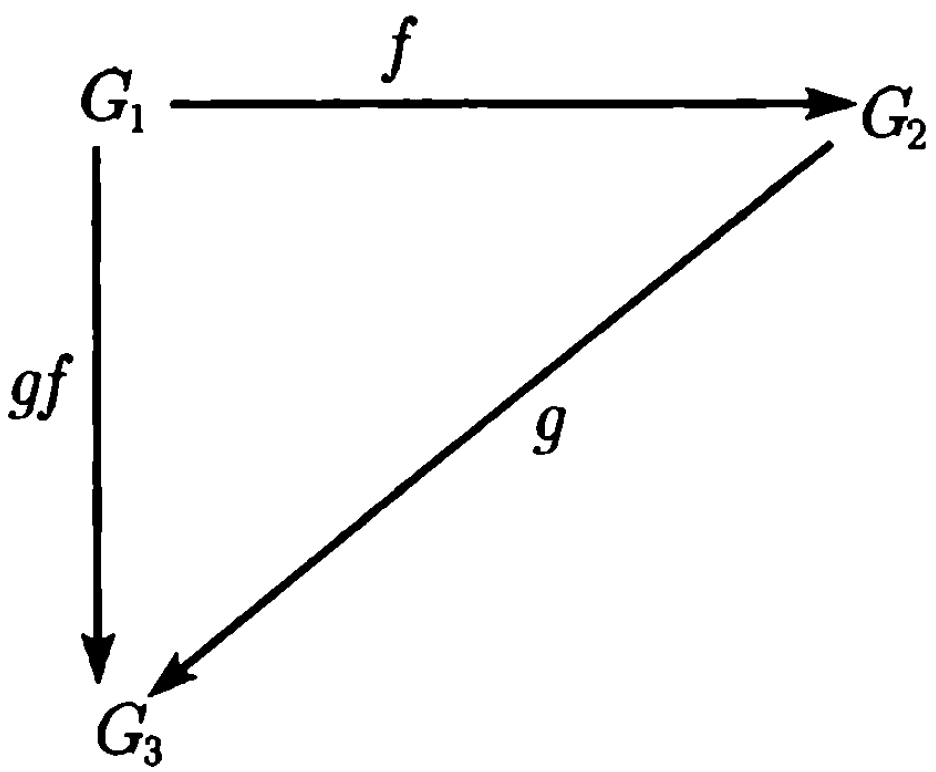
\includegraphics[scale=0.2]{交换图2.png}
\caption{}
\label{figure:{交换图2}}
\end{figure}
\begin{proof}
\begin{enumerate}[(1)]
\item 事实上, \( \forall a,b \in G_1 \) 有 \( gf(a), gf(b) \in G_3 \) 且
\[
gf(ab) = g(f(ab)) = g(f(a)f(b)) = gf(a)gf(b).
\]
故 \( gf \) 为 \( G_1 \) 到 \( G_3 \) 的同态. 又由 \( f(G_1) = G_2, g(G_2) = G_3 \), 即得 \( gf(G_1) = G_3 \). 又由 \( g,f \) 为一一对应, 则 \( gf \) 也是一一对应.

\item 事实上, \( f(e_1) = f(e_1^2) = f(e_1)f(e_1) \), 故有
\[
f(e_1) = f(e_1)f(e_1)^{-1} = e_2.
\]
又 \( a \in G_1 \) 有 \( f(e_1) = f(aa^{-1}) = f(a)f(a^{-1}) \), 故
\[
f(a^{-1}) = f(a)^{-1}f(e_1) = f(a)^{-1}.
\]

\item 事实上, 由性质(2)知 \( e_2 = f(e_1) \in f(G_1) \), 又 \( f(a),f(b) \in f(G_1) \) 有 \( f(a)f(b)^{-1} = f(ab^{-1}) \in f(G_1) \), 故 \( f(G_1) \) 是 \( G_2 \) 的子群.

\item 对任何群 \( G \) 有 \( G \cong G \) (只要取 \( f = \text{id}_G \)); 若 \( G_1 \cong G_2 \), 则 \( G_2 \cong G_1 \) (若 \( f: G_1 \to G_2 \) 为同构映射, 则 \( f^{-1}: G_2 \to G_1 \) 也是同构映射); 若 \( G_1 \cong G_2, G_2 \cong G_3 \), 则 \( G_1 \cong G_3 \) (参见性质(1)).
\end{enumerate}
\end{proof}

\begin{definition}
设 \( G \) 是群. 对于 \( a \in G \), 可定义 \( G \) 的两个变换 \( L_a, R_a \) 如下:
\[
L_a(x) = ax, \quad R_a(x) = xa, \quad \forall x \in G.
\]
\( L_a, R_a \) 分别称为由 \( a \) 决定的\textbf{左平移}与\textbf{右平移}.定义
\begin{align*}
L_G\triangleq \{L_a|a\in G\},\quad R_G\triangleq \{R_a|a\in G\}.
\end{align*}
\end{definition}

\begin{proposition}
$G$上由$a$决定的左平移,右平移\( L_a, R_a \) 都是 \( G \) 的一一对应, 即为 \( S_G \) 中元素且有
\begin{align*}
L_aL_b &= L_{ab}, \quad R_aR_b = R_{ba}, \quad L_1 = R_1 = \text{id}_G, \\
L_{a^{-1}} &= L_a^{-1}, \quad R_{a^{-1}} = R_a^{-1}, \quad L_aR_b = R_bL_a, \quad \forall a,b \in G,
\end{align*}
\( 1 \) 为 \( G \) 的幺元.从这些等式可知 \( L_G = \{L_a|a \in G\} \) 与 \( R_G = \{R_a|a \in G\} \) 都是 \( S_G \) 的子群.
\end{proposition}
\begin{proof}

\end{proof}

\begin{theorem}[Cayley定理]\label{theorem:抽象代数-Cayley定理-定理 1.5.1}
设 \( G \) 是一个群, 则
\[
G \cong L_G \cong R_G.
\]
\end{theorem}
\begin{remark}
左平移与右平移的概念对半群与幺半群也是适用的. 但应注意, 此时左右平移不一定是一一对应.Cayley 定理对半群是不成立的, 但对幺半群 \( G \) 仍有 \( G \cong L_G \), 这时 \( L_G \) 是 \( M(G) \) 的子幺半群 (\( M(G) \) 的定义见\refexa{example:抽象代数-例题1.2.2}).
\end{remark}
\begin{proof}
记 \( G \) 到 \( L_G \) 的映射 \( L: L(a) = L_a \). 显然 \( L \) 是满映射. 又若 \( L(a) = L(b) \), 即 \( L_a = L_b \), 则有 \( a = a \cdot 1 = L_a(1) = L_b(1) = b \), 因而 \( L \) 还是一一映射, 故 \( L \) 为一一对应. 又对 \( \forall a,b \in G \) 有
\[
L(ab) = L_{ab} = L_aL_b = L(a)L(b),
\]
故 \( L \) 是 \( G \) 到 \( L_G \) 上的同构, 即 \( G \cong L_G \).

类似地, 不难验证, 由 \( R'(a) = R_{a^{-1}} \) 确定的 \( G \) 到 \( R_G \) 的映射 \( R' \) 也是一个同构, 即有 \( G \cong L_G \cong R_G \).
\end{proof}

\begin{definition}
群 \( G \) 到自身的同构称为 \( G \) 的\textbf{自同构}, 群 \( G \) 的自同构的集合记为 \( \text{Aut}G \).
\end{definition}

\begin{theorem}
设 \( G \) 是一个群, 则有
\begin{enumerate}[(1)]
\item \( \text{Aut}G \) 对变换的乘法也是一个群, 称为 \( G \) 的\textbf{自同构群};
\item \( \forall g \in G \), \( G \) 的变换 \( \text{ad}g = L_gR_{g^{-1}} \) 是 \( G \) 的一个自同构, 称为由 \( g \) 决定的\textbf{内自同构};
\item \( G \) 的内自同构的集合 \( \text{Int}G \) (也记成 \( \text{ad}G \)) 是 \( \text{Aut}G \) 的正规子群, 称为 \( G \) 的\textbf{内自同构群};
\item \( \text{ad}: g \to \text{ad}g \) 是群 \( G \) 到 \( \text{Int}G \) 上的同态.
\end{enumerate}
\end{theorem}
\begin{proof}
\begin{enumerate}[(1)]
\item 显然有 \( \text{id}_G \in \text{Aut}G \subseteq S_G \), 任取 \( \theta_1, \theta_2 \in \text{Aut}G \), 于是 \( \theta_1\theta_2^{-1} \in S_G \) 且对 \( \forall x,y \in G \),
\begin{align*}
\theta_1\theta_2^{-1}(xy) &= \theta_1(\theta_2^{-1}(xy)) = \theta_1(\theta_2^{-1}(\theta_2\theta_2^{-1}(x) \cdot \theta_2\theta_2^{-1}(y))) \\
&= \theta_1(\theta_2^{-1}\theta_2(\theta_2^{-1}(x)\theta_2^{-1}(y))) = \theta_1(\theta_2^{-1}(x)\theta_2^{-1}(y)) \\
&= \theta_1\theta_2^{-1}(x) \cdot \theta_1\theta_2^{-1}(y),
\end{align*}
即有 \( \theta_1\theta_2^{-1} \in \text{Aut}G \). 故 \( \text{Aut}G \) 是群.

\item 对 \( \forall g \in G \) 有 \( L_g, R_{g^{-1}} \in S_G \), 因而 \( \text{ad}g = L_gR_{g^{-1}} \in S_G \), 又对 \( \forall x,y \in G \), 有
\[
\text{ad}g(xy) = g(xy)g^{-1} = (gxg^{-1})(gyg^{-1}) = \text{ad}g(x) \cdot \text{ad}g(y).
\]
故 \( \text{ad}g \in \text{Aut}G \), 即 \( \text{ad}g \) 是 \( G \) 的自同构.

\item 对 \( \forall g_1,g_2 \in G \), 有
\begin{align}
(\text{ad}g_1)(\text{ad}g_2)^{-1} &= L_{g_1}R_{g_1^{-1}}(L_{g_2}R_{g_2^{-1}})^{-1} \nonumber \\
&= L_{g_1}R_{g_1^{-1}}R_{g_2}L_{g_2^{-1}} = L_{g_1}L_{g_2^{-1}}R_{g_1^{-1}}R_{g_2} \nonumber \\
&= L_{(g_1g_2^{-1})}R_{(g_2g_1^{-1})} = \text{ad}g_1g_2^{-1}. \label{eq:1.5.1}
\end{align}
故 \( \text{Int}G \) 是 \( \text{Aut}G \) 的子群.

又对 \( \forall g,a \in G \), \( \forall \theta \in \text{Aut}G \),
\[
\theta(\text{ad}g)\theta^{-1}(a) = \theta(g\theta^{-1}(a)g^{-1}) = \theta(g)a\theta(g)^{-1} = \text{ad}\theta(g)(a),
\]
因而
\[
\theta(\text{ad}g)\theta^{-1} = \text{ad}\theta(g), \quad \forall g \in G, \theta \in \text{Aut}G. \label{eq:1.5.2}
\]
由此知 \( \text{Int}G \) 是 \( \text{Aut}G \) 的正规子群.

\item 在式 \(\eqref{eq:1.5.1}\) 中, 取 \( g_1 = 1 \), 则有
\[
(\text{ad}g_2)^{-1} = \text{ad}g_2^{-1}.
\]
一般由式 \(\eqref{eq:1.5.1}\) 知
\[
\text{ad}g_1 \cdot \text{ad}g_2 = (\text{ad}g_1)(\text{ad}g_2)^{-1})^{-1} = \text{ad}g_1(g_2^{-1})^{-1} = \text{ad}g_1g_2.
\]
由此知 \( \text{ad}: G \to \text{Int}G \) 为 \( G \) 到 \( \text{Int}G \) 上的同态映射.
\end{enumerate}
\end{proof}

\begin{definition}
设 \( G \) 是一个群, \( \text{Aut}G, \text{Int}G \) 分别为 \( G \) 的自同构群与内自同构群, 称商群 \( \text{Aut}G/\text{Int}G \) 为 \( G \) 的\textbf{外自同构群}.
\end{definition}

\begin{definition}
设 \( R, R_1 \) 是两个环, \( \varphi \) 是 \( R \) 到 \( R_1 \) 的映射, 如果对 \( \forall a,b \in R \),
\[
\varphi(a + b) = \varphi(a) + \varphi(b),
\]
\[
\varphi(ab) = \varphi(a)\varphi(b),
\]
那么称 \( \varphi \) 是 \( R \) 到 \( R_1 \) 的一个\textbf{同态}.

若 \( \varphi \) 是满映射, 则称 \( \varphi \) 为\textbf{满同态}, 或称\( \varphi \) 为 \( R \) 到 \( R_1 \) 上的同态.

若 \( \varphi \) 还是一一对应, 则称 \( \varphi \) 为\textbf{同构}. 这时也称 \( R \) 与 \( R_1 \) 同构, 记为 \( R \cong R_1 \).
\end{definition}

\begin{proposition}
\begin{enumerate}
\item 若 \( \varphi \) 是 \( R \) 到 \( R_1 \) 的同态, 则\( \varphi(R) \) 是 \( R_1 \) 的子环. 

\item 环的同态的积还是环同态. 

\item 环的同构关系是等价关系, 即 \( R \cong R; R \cong R_1 \Rightarrow R_1 \cong R; R_1 \cong R_2, R_2 \cong R_3 \Rightarrow R_1 \cong R_3 \).
\end{enumerate}
\end{proposition}
\begin{proof}
\begin{enumerate}
\item 

\item 

\item 
\end{enumerate}
\end{proof}

\begin{example}
设 \( R, R_1 \) 是两个环. 定义 \( R \) 到 \( R_1 \) 的映射 \( \varphi: \varphi(x) = 0 (\forall x \in R) \), 则 \( \varphi \) 为 \( R \) 到 \( R_1 \) 的同态, 这样的同态称为\textbf{零同态}.
\end{example}
\begin{proof}

\end{proof}

\begin{example}
设 \( I \) 是环 \( R \) 的一个理想. \( R \) 到商环 \( R/I \) 的自然映射 \( \pi: \pi(x) = x + I (\forall x \in R) \) 是 \( R \) 到 \( R/I \) 上的同态, 称为\textbf{自然同态}.
\end{example}
\begin{proof}

\end{proof}

\begin{example}
设 \( V \) 是数域 \( P \) 上 \( n \) 维线性空间, 用 \( \text{End}V \) 表示 \( V \) 上线性变换的集合, 显然, \( \text{End}V \) 对线性变换的加法与乘法构成一环, 设 \( \{\alpha\} = \{\alpha_1, \alpha_2, \cdots, \alpha_n\} \) 是 \( V \) 的一组基, 则映射
\[
\mathcal{A} \to M(\mathcal{A}), \quad \forall \mathcal{A} \in \text{End}V
\]
是 \( \text{End}V \) 到 \( P^{n \times n} \) 上的同构.这里$M(\mathcal{A})$表示线性变换基$\{\alpha\}$下的矩阵.
\end{example}
\begin{proof}

\end{proof}

\begin{definition}
设 \( R, R' \) 是两个环, 若 \( R \) 到 \( R' \) 的映射 \( \varphi \), 对 \( \forall a,b \in R \) 满足
\[
\varphi(a + b) = \varphi(a) + \varphi(b), \quad \varphi(ab) = \varphi(b)\varphi(a),
\]
则称 \( \varphi \) 是从 \( R \) 到 \( R' \) 的\textbf{反同态}. 又若 \( \varphi \) 还是一一对应, 则称 \( \varphi \) 为从 \( R \) 到 \( R' \) 的\textbf{反同构}.

一个环 \( R \) 到自身的反同构称为\textbf{反自同构}. 若环 \( R \) 的反自同构 \( \eta \) 满足 \( \eta^2 = \text{id}_R \), 则称 \( \eta \) 为 \( R \) 的一个\textbf{对合}.
\end{definition}

\begin{theorem}
对任一环 \( R \), 一定有一个环 \( R' \) 与它反同构.
\end{theorem}
\begin{proof}
事实上, 只需作一个与 \( R \) 一一对应的集合 \( R' \), 设映射 \( x \to x' \) 为这个对应关系. 在 \( R' \) 中定义加法与乘法如下:
\[
x' + y' = (x + y)', \quad x'y' = (yx)', \quad \forall x', y' \in R',
\]
则 \( R' \) 成环且与 \( R \) 反同构.
\end{proof}

\begin{example}
设 \( P \) 是一个数域, 在环 \( P^{n \times n} \) 中定义映射 \( \tau: A \to A' \), 则 \( \tau \) 是 \( P^{n \times n} \) 的对合.
\end{example}
\begin{proof}

\end{proof}


































\end{document}